\documentclass[12pt,titlepage]{article}
\usepackage{geometry}

\usepackage[utf8]{inputenc}
\usepackage[greek,english]{babel}
\usepackage{alphabeta}
\usepackage[T1]{fontenc}

\usepackage{graphicx}
\graphicspath{{../plots/}}

\usepackage{tikz}
\usetikzlibrary{graphs}
\usetikzlibrary{automata}
\tikzset{->,node distance=2cm}

\usepackage{booktabs}

\begin{document}

\title{Συστήματα Παράλληλης Επεξεργασίας\\
    Άσκηση 1\\
    Τελική Αναφορά}
\author{Αλέξιος Ζαμάνης\\
    03115010\\
    Παναγιώτης Ζώγας\\
    03115191}
\date{18 Νοεμβρίου 2019}

\maketitle

\section{Conway's Game of Life}

Στο πρώτο κομμάτι της άσκησης παραλληλοποιούμε την υλοποίηση του Conway's Game
of Life. Ουσιαστικά πρόκειται για 3 εμφωλευμένους βρόχους, 1 για το χρόνο και 2
για τις χωρικές συντεταγμένες. Δεδομένου ότι η κατάσταση ενός κελιού κάθε χρονική
στιγμή εξαρτάται (άμεσα ή έμμεσα) από την κατάσταση όλου του ταμπλό τις
προηγούμενες χρονικές στιγμές, δε διακρίνουμε παραλληλία στον αξονα του χρόνου.
Αντίθετα, για μια χρονική στιγμή τα κελιά δεν εμφανίζουν χωρικές εξαρτήσεις,
ήτοι δεν εξαρτώνται από την τωρινή κατάσταση των υπόλοιπων κελιών, οπότε έχουμε
δυνατότητα παράλληλης εκτέλεσης και στους 2 άξονες, ήτοι σε επίπεδο κελιού.

Ιδανικά θέλουμε να τρέξουμε N\textsuperscript2 παράλληλους υπολογισμούς, όπου N
το μέγεθος του ταμπλό. Αυτό στο OpenMP εκφράζεται ως εξής:

\begin{verbatim}
#pragma omp parallel for collapse(2) default(none) private(nbrs) \
shared(N, current, previous)
for (i = 1; i < N - 1; i++) 
    for (j = 1; j < N - 1; j++) {...}
\end{verbatim}

Ήτοι ζητάμε κατανομή της εργασίας των 2 for loops μεταξύ των νημάτων που
δημιουργούμε με το directive parallel (το πλήθος τους καθορίζεται στο runtime
με το environment variable OMP\_NUM\_THREADS). Χρήσει του collapse τα 2 for
loops νοούνται ως ένα με (N-1)\textsuperscript{2} επαναλήψεις. Επιπλέον ζητάμε
ιδιωτικά αντίγραφα implicitly για τους indexes (i και j) και explicitly για την
προσωρινή μεταβλητή που μετράει τους ζωντανούς γείτονες (nbrs). Αντίθετα,
επιτρέπουμε στις N και previous να είναι κοινές, καθώς δεν τις μεταβάλλουμε,
όπως και στην current, της οποίας κάθε στοιχείο μεταβάλλεται από διαφορετικό
νήμα (οπότε δεν έχουμε race conditions).

Δεδομένου όμως ότι διαθέτουμε το πολύ 8 πυρήνες για την παράλληλη εκτέλεση, δεν
έχει νόημα αυτός ο βαθμός παραλληλοποίησης. Παραλληλοποιούμε λοιπόν σε επίπεδο
γραμμής, ισοκατανέμοντας τον φόρτο του κάθε νήματος. Χρήσει του OpenMP έχουμε:

\begin{verbatim}
#pragma omp parallel for default(none) private(j, nbrs) \
shared(N, current, previous)
for (i = 1; i < N - 1; i++) {...}
\end{verbatim}

Σημειώνουμε ότι εδώ χρειάζεται να δηλώσουμε ρητά ότι ο index j πρέπει να είναι
private.

Εκτελώντας τις δύο παραπάνω εκδοχές παρατηρούμε, όπως αναμέναμε, μηδαμινή αλλαγή
στους χρόνους εκτέλεσης. Ως εκ τούτου, επιλέγουμε ως βέλτιστη υλοποίηση τη
δεύτερη.

Παραθέτουμε παρακάτω τα διαγράμματα του χρόνου εκτέλεσης ως προς τον πλήθος των
νημάτων για κάθε μέγεθος του ταμπλό.

\begin{center}
    \includegraphics[width=.49\textwidth]{ask1/time-64}
    \includegraphics[width=.49\textwidth]{ask1/time-1024}
    \includegraphics[width=.49\textwidth]{ask1/time-4096}
\end{center}

Επιπλέον δίνουμε ένα διάγραμμα του speedup ως προς το πλήθος των νημάτων για όλα
τα μεγέθη του ταμπλό (βλέπε επόμενη σελίδα).

Εύκολα παρατηρούμε ότι μόνο για ταμπλό μεγέθους 1024 έχουμε γραμμικό speedup.
Αντίθετα, για τα υπόλοιπα μεγέθη η βελτίωση του χρόνου εκτέλεσης φαίνεται να
κορέννυται μετά από κάποιο κατώφλι. Συγκεκριμένα, για το μεγάλο ταμπλό το
speedup παύει να αυξάνεται γραμμικά για πάνω από 4 νήματα και τελικά φτάνει
κοντά στο 5, ενώ για το μικρό ταμπλό δεν ξεπερνά το 2.5 (μάλιστα για 8 νήματα
μειώνεται).

Για το μικρό ταμπλό ο χρόνος εκτέλεσης του σειριακού προγράμματος είναι ήδη πολύ
μικρός. Επομένως εικάζουμε πως το κόστος της κατασκευής και της διαχείρισης των
νημάτων είναι συγκρίσιμο με το χρόνο εκτέλεσης. Μάλιστα όσο αυξάνουμε το πλήθος
των νημάτων, τόσο μεγαλύτερο το κόστος και τοσο λιγότερη η δουλειά που έχει να
εκτελέσει το καθένα. Για 8 νήματα το καθένα θα αναλάβει περίπου 8 στήλες, ήτοι
ασήμαντη υπολογιστικά δουλειά. Έτσι στο συνολικό χρόνο εκτέλεσης θα καταλήγει να
κυριαρχεί ο νεκρός χρόνος.

Για το μεγάλο ταμπλό η μεταφορά του από τη μνήμη γίνεται κοστοβόρα, ενώ πιθανόν
να μη χωράει το ταμπλό (ή τα κομμάτια του) στην cache και να μεταφέρονται σε
κάθε επανάληψη. Παράλληλα, αυξάνοντας τα νήματα διαμοιράζεται ο υπολογιστικός
κόπος, με αποτέλεσμα το πρόγραμμα να γίνεται memory bound. Εν αγνοία των μεγεθών
της cache, εικάζουμε πως από 4 νήματα και πάνω το memory intensity είναι αρκετό,
ώστε να αναχαιτίσει τα οφέλη του πολυνηματισμού.

\begin{center}
    \includegraphics[width=\textwidth]{ask1/speedup}
\end{center}

\newpage

\section{Παραλληλοποίηση και βελτιστοποίηση του\\ αλγορίθμου Floyd-Warshall σε αρχιτεκτονικές\\ κοινής μνήμης}

\subsection{Standard Floyd-Warshall}

Στο δεύτερο και κύριο τμήμα της εργασίας μελετάμε τον αλγόριθμο Floyd-Warshall,
καθώς και κάποιες παραλλαγές του, που στοχεύουν στην καλύτερη αξιοποίηση της
cache.

Στην απλούστερη εκδοχή του ο αλγόριθμος αποτελείται από 3 εμφωλευμένους βρόχους.
Ο εξωτερικός βρόχος αναπαριστά το χρόνο k και οι 2 εσωτερικοί τις χωρικές
συντεταγμένες i και j. Για δεδομένη αρίθμηση των κόμβων του γράφου, στην k-οστη
επανάληψη του εξωτερικού βρόχου υπολογίζονται τα συντομότερα μονοπάτια που
χρησιμοποιούν ως ενδιάμεσους κόμβους κάποιους εκ των 1 έως k.

Δεδομένου ότι απαγορεύονται τα self loops, τα διαγώνια στοιχεία του πίνακα
αρχικοποιούνται στο 0. Ως εκ τούτου, βελτίωσή τους, ήτοι αρνητική τιμή σε
διαγώνιο στοιχείο, ισοδυναμεί με εύρεση αρνητικού κύκλου, στην οποία περίπτωση η
έννοια των συντομότερων μονοπατιών δεν έχει νόημα. Μπορούμε λοιπόν να θεωρήσουμε
ότι στις περιπτώσεις ενδιαφέροντος τα διαγώνια στοιχεία θα παραμένουν 0. Ως εκ
τούτου, στην k-οστή επανάληψη, τα στοιχεία της k-οστής γραμμής ή στήλης δε θα
μεταβάλλονται.

Από τα παραπάνω βλέπουμε εύκολα ότι στην k-οστή επανάληψη συγκρίνουμε το
στοιχείο A\textsubscript{ij} με τον εαυτό του και με τα A\textsubscript{ik}
και A\textsubscript{kj}, που θα παραμείνουν σταθερά, επομένως δεν υπαρχουν
πραγματικές χωρικές εξαρτήσεις. Δικαιούμαστε λοιπόν να παραλληλοποιήσουμε πλήρως
τους 2 χωρικούς βρόχους.

Συμπεραίνουμε πως κάθε στοιχείο εξαρτάται από (το πολύ) 3 προηγούμενα στοιχεία.
Για την περίπτωση ενός 2$\times$2 πίνακα έχουμε 2 επαναλήψεις με τις εξαρτήσεις
που φαίνονται στο ακόλουθο σχήμα. Εύκολα γίνεται αντιληπτή η γενίκευση σε N
στοιχεία.

\begin{center}
    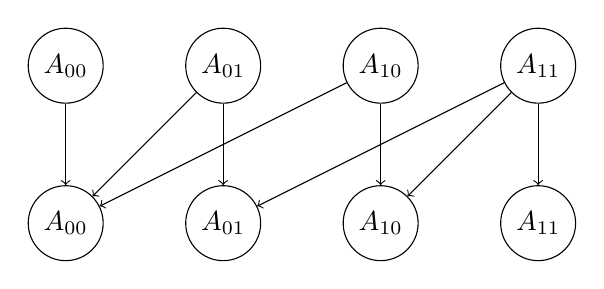
\begin{tikzpicture}
        \node[state] (00) {$A_{00}$};
        \node[state, right of=00] (01) {$A_{01}$};
        \node[state, right of=01] (10) {$A_{10}$};
        \node[state, right of=10] (11) {$A_{11}$};
        \node[state, below of=00] (00') {$A_{00}$};
        \node[state, right of=00'] (01') {$A_{01}$};
        \node[state, right of=01'] (10') {$A_{10}$};
        \node[state, right of=10'] (11') {$A_{11}$};
        \draw (00) edge (00')
        (01) edge (00')
        (10) edge (00')
        (01) edge (01')
        (11) edge (01')
        (10) edge (10')
        (11) edge (10')
        (11) edge (11');
    \end{tikzpicture}
\end{center}

Δεδομένης της έλλειψης χωρικών εξαρτήσεων, μπορούμε να παραλληλοποιήσουμε και τα
2 for loops, νοώντας τα ως ένα. Στο OpenMP έχουμε:

\begin{verbatim}
#pragma omp parallel for collapse(2) default(none) shared(A, k, N)
for (i = 0; i < N; i++)
    for (j = 0; j < N; j++) {...}
\end{verbatim}

Εναλλακτικά μπορούμε να παραλληλοποιήσουμε μόνο τον εξωτερικό βρόχο. Στο OpenMP
έχουμε:

\begin{verbatim}
#pragma omp parallel for default(none) private(j) shared(A, k, N)
for (i = 1; i < N; i++) {...}
\end{verbatim}

Όπως και στην προηγούμενη ενότητα, παρατηρούμε ότι ο βαθμός παραλληλοποίησης
του εξωτερικού loop επαρκεί για το δοσμένο αριθμό νημάτων. Ως εκ τούτου, δεν
βελτιώνεται ο χρόνος χρήσει του collapse (μάλιστα χειροτερεύει με ελάχιστες
εξαιρέσεις), οπότε πάλι προτιμούμε τη δεύτερη υλοποίηση.

Ακολουθούν διαγράμματα του χρόνου εκτέλεσης και του speedup συναρτήσει του
πλήθους των χρησιμοποιούμενων threads.

\begin{center}
    \includegraphics[width=.49\textwidth]{ask2/openmp/fw-time-1024}
    \includegraphics[width=.49\textwidth]{ask2/openmp/fw-time-2048}
    \includegraphics[width=.49\textwidth]{ask2/openmp/fw-time-4096}
    \includegraphics[width=.49\textwidth]{ask2/openmp/fw-speedup}
\end{center}

Οι βέλτιστοι χρόνοι για τα διάφορα μεγέθη πινάκων είναι οι εξής:

\begin{center}
    \begin{tabular}{@{}lll@{}}
        \toprule
        N    & Number of threads & Time    \\
        \midrule
        1024 & 16                & 0.2166  \\
        2048 & 32                & 1.38116 \\
        4096 & 16                & 17.6027 \\
        \bottomrule
    \end{tabular}
\end{center}

Εύκολα παρατηρούμε ότι η υλοποίηση κλιμακώνει σχεδόν γραμμικά μέχρι 8 νήματα,
υπογραμμικά μέχρι τα 16 (για N=2048 μέχρι τα 32) και στη συνέχεια η επίδοση είτε
παύει να βελτιώνεται είτε χειροτερεύει. Από τα παραπάνω συμπεραίνουμε ότι το
πρόβλημα είναι memory bound, ήτοι εκτελεί πολύ απλούς υπολογισμούς σε πολλά
δεδομένα. Επομένως χωρίς βέλτιστη χρήση της cache η παραλληλοποίησή του μπορεί
να αποβεί ακόμα και κοστοβόρα.

\newpage

\subsection{Recursive Floyd-Warshall}

Στοχεύοντας στη βέλτιστη εκμετάλλευση της cache διαιρούμε τον πίνακα σε blocks
κατάλληλου μεγέθους και εκτελούμε αναδρομικά (ή επαναληπτικά) τον
Floyd-Warshall σε καθένα από αυτά. Πλέον δηλαδή το A\textsubscript{ij}
δηλώνει block αντί για στοιχείο.

Δυστυχώς η υπόθεση μας για διατήρηση της τιμής των στοιχείων με i=k ή j=k παύει
να ισχύει. Ως εκ τούτου, πρέπει να επιβάλουμε μια σειρά στις λειτουργίες όπως
απαιτούν οι εξαρτήσεις. Πρώτα υπολογίζουμε το A\textsubscript{kk}, έπειτα τα
A\textsubscript{ik} και Α\textsubscript{jk} βάσει του πρώτου και τέλος τα
A\textsubscript{ij} βάσει των προηγουμένων. Για N=2 έχουμε το παρακάτω σχήμα:

\begin{center}
    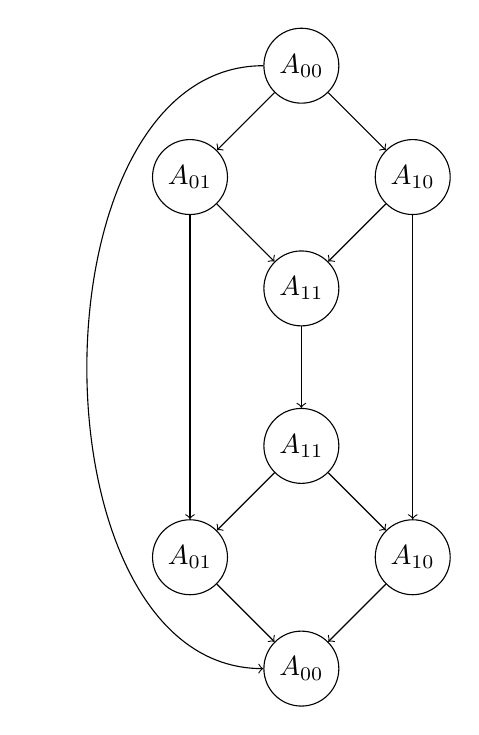
\begin{tikzpicture}
        \node[state] (00) {$A_{00}$};
        \node[state, below left of=00] (01) {$A_{01}$};
        \node[state, below right of=00] (10) {$A_{10}$};
        \node[state, below right of=01] (11) {$A_{11}$};
        \node[state, below of=11] (11') {$A_{11}$};
        \node[state, below left of=11'] (01') {$A_{01}$};
        \node[state, below right of=11'] (10') {$A_{10}$};
        \node[state, below right of=01'] (00') {$A_{00}$};
        \draw (00) edge (01)
        (00) edge (10)
        (01) edge (11)
        (10) edge (11)
        (11) edge (11')
        (01) edge (01')
        (11') edge (01')
        (10) edge (10')
        (11') edge (10')
        (00) edge[bend right=90] (00')
        (01') edge (00')
        (10') edge (00');
    \end{tikzpicture}
\end{center}

Διακρίνουμε 2 επαναλήψεις με 3 στάδια έκαστη, εκ των οποίων το 2ο και το 3ο
έχουν 2 και στη γενική περίπτωση πολλές ανεξάρτητες συνιστώσες. Η εικονιζόμενη
περίπτωση αντιστοιχεί σε μια αναδρομική κλήση του recursive αλγορίθμου και
αποτελεί ειδική περίπτωση του tiled για N=2. Εύκολα προκύπτει από το σχήμα και
την προηγηθείσα συζήτηση η γενίκευση για μεγαλύτερα N.

Όσον αφορά την υλοποίηση, η recursive εκδοχή επιβάλλει, λόγω της αναδρομής,
υλοποίηση με tasks. Η υλοποίηση στο OpenMP έχει ως εξής:

\begin{verbatim}
#pragma omp parallel default(none) shared(A, B, N)
#pragma omp single
FW_SR(A, 0, 0, A, 0, 0, A, 0, 0, N, B);
...
FW_SR(A, arow, acol, B, brow, bcol,
    C, crow, ccol, myN / 2, bsize);
#pragma omp task
FW_SR(A, arow, acol + myN / 2, B, brow, bcol,
    C, crow, ccol + myN / 2, myN / 2, bsize);
#pragma omp task
FW_SR(A, arow + myN / 2, acol, B, brow + myN / 2, bcol,
    C, crow, ccol, myN / 2, bsize);
#pragma omp taskwait
FW_SR(A, arow + myN / 2, acol + myN / 2, B, brow + myN / 2, bcol,
    C, crow, ccol + myN / 2, myN / 2, bsize);
FW_SR(A, arow + myN / 2, acol + myN / 2, B, brow + myN / 2, bcol + myN / 2,
    C, crow + myN / 2, ccol + myN / 2, myN / 2, bsize);
#pragma omp task
FW_SR(A, arow + myN / 2, acol, B, brow + myN / 2, bcol + myN / 2,
    C, crow + myN / 2, ccol, myN / 2, bsize);
#pragma omp task
FW_SR(A, arow, acol + myN / 2, B, brow, bcol + myN / 2,
    C, crow + myN / 2, ccol + myN / 2, myN / 2, bsize);
#pragma omp taskwait
FW_SR(A, arow, acol, B, brow, bcol + myN / 2,
    C, crow + myN / 2, ccol, myN / 2, bsize);
\end{verbatim}

Δημιουργούμε το thread pool κατά την πρώτη αναδρομική κλήση, την οποία εκτελεί
μόνο 1 νήμα. Το νήμα αυτό (και κάθε άλλο νήμα που καλεί αναδρομικά τη συνάρτηση)
αναλαμβάνει να εκτελέσει ορισμένες αναδρομικές κλήσεις και να δημιουργήσει tasks
με κάποιες άλλες (\#pragma omp task), τα οποία στη συνέχεια θα περιμένει
(\#pragma omp taskwait) πριν συνεχίσει, όπως επιβάλλουν οι εξαρτήσεις του
αλγορίθμου.

Ύστερα από μετρήσεις για διάφορες τιμές του B, βρίσκουμε ότι οι βέλτιστοι χρόνοι
εκτέλεσης προκύπτουν για B=64 και B=128, που αντιστοιχούν στη βέλτιστη
αξιοποίηση της L1 και της L2 cache αντίστοιχα. Οι παραπάνω τιμές προκύπτουν και
θεωρητικά, αν σκεφτούμε ότι κάθε block έχει μέγεθος
B\textsuperscript2*sizeof(int), όπου sizeof(int)=4, και ζητάμε το μέγιστο B
τέτοιο, ώστε το μέγεθος του block να μην ξεπερνά το μέγεθος της (μισής) cache (32
KiB για την L1 και 256 KiB για την L2). Υποθέτουμε απλοποιητικά εδώ ότι στην
περίπτωση που έχουμε 64 νήματα, οπότε κάθε πυρήνας στεγάζει 2 νήματα, καθένα
χρησιμοποιεί τη μισή cache.

Παραθέτουμε παρακάτω τις μετρήσεις χρόνου εκτέλεσης και speedup συναρτήσει του
αριθμού των νημάτων για B=64.

\begin{center}
    \includegraphics[width=.49\textwidth]{ask2/openmp/fw_sr-64-time-1024}
    \includegraphics[width=.49\textwidth]{ask2/openmp/fw_sr-64-time-2048}
    \includegraphics[width=.49\textwidth]{ask2/openmp/fw_sr-64-time-4096}
    \includegraphics[width=.49\textwidth]{ask2/openmp/fw_sr-64-speedup}
\end{center}

Ομοίως για B=128:

\begin{center}
    \includegraphics[width=.49\textwidth]{ask2/openmp/fw_sr-128-time-1024}
    \includegraphics[width=.49\textwidth]{ask2/openmp/fw_sr-128-time-2048}
    \includegraphics[width=.49\textwidth]{ask2/openmp/fw_sr-128-time-4096}
    \includegraphics[width=.49\textwidth]{ask2/openmp/fw_sr-128-speedup}
\end{center}

Οι βέλτιστοι χρόνοι για τα διάφορα μεγέθη πινάκων είναι οι εξής:

\begin{center}
    \begin{tabular}{@{}llll@{}}
        \toprule
        N    & B  & Number of threads & Time    \\
        \midrule
        1024 & 64 & 8                 & 0.3349  \\
        2048 & 64 & 16                & 2.0179  \\
        4096 & 64 & 16                & 11.4688 \\
        \bottomrule
    \end{tabular}
\end{center}

Παρατηρούμε ότι ο βέλτιστος χρόνος για Ν=4096 μειώθηκε αισθητά (οι άλλοι
αυξήθηκαν). Επομένως υπάρχει πράγματι βελτίωση για μεγάλους πίνακες, που
υποφέρουν από κακό locality. Δυστυχώς είναι εμφανές ότι η υλοποίησή μας δεν
κλιμακώνει όπως θα θέλαμε. Η (αισθητά υπογραμμική) κλιμάκωση σταματά στα 16
threads (για N=1024 στα 4 ή 8 threads), ενώ για πιο μεγάλες τιμές η επίδοση μόνο
χειροτερεύει.

Μια εναλλακτική υλοποίηση δε δημιουργεί το 2ο και το 4ο task (όπως αυτά
φαίνονται στον προηγούμενο κώδικα), με το σκεπτικό ότι το νήμα που δημιουργεί τα
tasks απλά θα περιμένει άεργο τα 2 tasks, ενώ θα μπορούσε να εκτελεί το 1 από
τα 2. Εντούτοις οι χρόνοι εκτέλεσης αυτής της υλοποίησης είναι πλέον χειρότεροι,
καθώς εντείνεται η ανισοκατανομή της εργασίας μεταξύ των threads. Μάλιστα, το
thread που εκτέλεσε την πρώτη αναδρομική κλήση φαίνεται να αναλαμβάνει αισθητά
μεγαλύτερο όγκο από όλα τα υπόλοιπα (όπως προκύπτει και από σχετικές μετρήσεις).

Συμπεραίνουμε πως η βέλτιστη πρακτική, όταν χρησιμοποιούνται τα tasks, είναι η
δημιουργία ενός task pool με πολλά tasks, ώστε να υπάρχει πάντοτε εργασία για
όλα τα threads.

\newpage

\subsection{Tiled Floyd-Warshall}

Απογοητευμένοι από τη μη κλιμακωσιμότητα της αναδρομικής υλοποίησης καταφεύγουμε
στην tiled εκδοχή. Η συγκεκριμένη εκδοχή φαίνεται η πιο υποσχόμενη, καθώς
επιτρέπει πολλές διαφορετικές υλοποιήσεις (δεν επιβάλλει τη χρήση tasks όπως η
αναδρομή). Επιπλέον, όπως εξηγήσαμε στη θεωρητική ανάλυση που προηγήθηκε, η
tiled αποτελεί κατά μία έννοια γενίκευση της recursive εκδοχής.

Αρχικά δοκιμάζουμε μια task centric προσέγγιση. Στην ουσία ο Floyd-Warshall σε
κάθε tile γίνεται ένα διαφορετικό task προς εκτέλεση από τα ελεύθερα threads. Η
δημιουργία και η αναμονή των tasks γίνεται σύμφωνα με τους περιορισμούς που
επιβάλλουν οι εξαρτήσεις. Στο OpenMP έχουμε τα εξής:

\begin{verbatim}
#pragma omp parallel default(none) shared(A, i, j, k, B, N)
#pragma omp single
{
    #pragma omp task
    FW(A, k, k, k, B);
    #pragma omp taskwait
    for (i = 0; i < k; i += B)
        #pragma omp task
        FW(A, k, i, k, B);
    for (i = k + B; i < N; i += B)
        #pragma omp task
        FW(A, k, i, k, B);
    for (j = 0; j < k; j += B)
        #pragma omp task
        FW(A, k, k, j, B);
    for (j = k + B; j < N; j += B)
        #pragma omp task
        FW(A, k, k, j, B);
    #pragma omp taskwait
    for (i = 0; i < k; i += B)
        for (j = 0; j < k; j += B)
            #pragma omp task
            FW(A, k, i, j, B);
    for (i = 0; i < k; i += B)
        for (j = k + B; j < N; j += B)
            #pragma omp task
            FW(A, k, i, j, B);
    for (i = k + B; i < N; i += B)
        for (j = 0; j < k; j += B)
            #pragma omp task
            FW(A, k, i, j, B);
    for (i = k + B; i < N; i += B)
        for (j = k + B; j < N; j += B)
            #pragma omp task
            FW(A, k, i, j, B);
}
\end{verbatim}

Το πρώτο ζεύγος task-taskwait θα μπορούσε να παραλειφθεί, αλλά μάθαμε
προηγουμένως ότι θέλουμε τα περισσότερα δυνατά tasks στο task pool μας.

Εν συνεχεία δοκιμάζουμε μια data centric προσέγγιση. Στην ουσία κατανέμουμε τις
εργασίες στα threads βάσει των for loops. Στο OpenMP έχουμε:

\begin{verbatim}
#pragma omp parallel default(none) shared(A, k, B, N)
{
    #pragma omp single
    FW(A, k, k, k, B);
    #pragma omp for nowait
    for (i = 0; i < k; i += B)
        FW(A, k, i, k, B);
    #pragma omp for nowait
    for (i = k + B; i < N; i += B)
        FW(A, k, i, k, B);
    #pragma omp for nowait
    for (j = 0; j < k; j += B)
        FW(A, k, k, j, B);
    #pragma omp for
    for (j = k + B; j < N; j += B)
        FW(A, k, k, j, B);
    #pragma omp for nowait private(j)
    for (i = 0; i < k; i += B)
        for (j = 0; j < k; j += B)
            FW(A, k, i, j, B);
    #pragma omp for nowait private(j)
    for (i = 0; i < k; i += B)
        for (j = k + B; j < N; j += B)
            FW(A, k, i, j, B);
    #pragma omp for nowait private(j)
    for (i = k + B; i < N; i += B)
        for (j = 0; j < k; j += B)
            FW(A, k, i, j, B);
    #pragma omp for private(j)
    for (i = k + B; i < N; i += B)
        for (j = k + B; j < N; j += B)
            FW(A, k, i, j, B);
}
\end{verbatim}

Το \#pragma omp single και το \#pragma omp for θέτουν implicit barriers στο
τέλος του block τους. Δεδομένου ότι οι εργασίες μέσα στις 2 τετράδες από for
loops μπορούν να εκτελεσθούν παράλληλα, χρησιμοποιούμε το nowait, για να
αποφύγουμε τον αχρείαστο συγχρονισμό.

Εκτελούμε τις 2 υλοποιήσεις και παρατηρούμε ότι η δεύτερη είναι πλέον ταχύτερη
(παρότι αμφότερες είναι σαφώς καλύτερες από τις προηγούμενες). Αυτό είναι
αναμενόμενο, δεδομένου ότι το πρόβλημα είναι αρκετά κανονικό και δεν επωφελείται
από την ευελιξία που προσφέρουν τα tasks.

Προσπαθούμε να βελτιστοποιήσουμε τη δεύτερη εκδοχή. Δοκιμάζουμε την εξής
υλοποίηση:

\begin{verbatim}
#pragma omp parallel default(none) shared(A, k, B, N)
{
    #pragma omp single
    FW(A, k, k, k, B);
    #pragma omp for nowait
    for (i = 0; i < N; i += B)
        if (i != k)
            FW(A, k, i, k, B);
    #pragma omp for
    for (j = 0; j < N; j += B)
        if (j != k)
            FW(A, k, k, j, B);
    #pragma omp for private(j)
    for (i = 0; i < N; i += B)
        for (j = 0; j < N; j += B)
            if (i != k && j != k)
                FW(A, k, i, j, B);
}
\end{verbatim}

Στην ουσία έχουμε ενώσει τα διαδοχικά for loops, φροντίζοντας να μην
επαναλαμβάνουμε υπολογισμούς. Η ιδέα είναι να παροτρύνουμε το OpenMP να σπάσει
τον πίνακα έτσι, ώστε κάθε socket να αναλάβει το ένα τέταρτο του συνολικού
πίνακα. Δεδομένου ότι στη χειρότερη περίπτωση έχουμε N=4096, βλέπουμε ότι
4096\textsuperscript2*sizeof(int)/4=16 MiB, δηλαδή το ένα τέταρτο του πίνακα
χωράει ακριβώς στην L3 cache. Επομένως είναι θεμιτό από άποψη τοπικότητας κάθε
socket να ασχοληθεί με το ένα τέτατρο του πίνακα και μόνο.

Πράγματι παρατηρούμε αισθητή βελτίωση στους χρόνους, οπότε πορευόμαστε με αυτή
την εκδοχή.

Μέχρι τώρα υπολογίζουμε σε κάθε βήμα το κεντρικό tile, συνεχίζουμε με το σταυρό
(την κρίσιμη γραμμή και στήλη) και τελειώνουμε με τα υπόλοιπα tiles. Δοκιμάζουμε
τώρα να προσεγγίσουμε το πρόβλημα κατά γραμμές. Υπολογίζουμε όπως πριν το
κεντρικό tile, αλλά τώρα υπολογίζουμε μόνο την κρίσιμη γραμμή (όχι και την
κρίσιμη στήλη). Κάθε νήμα που θέλει να υπολογίσει μια γραμμή πρέπει πρώτα να
υπολογίσει το στοιχείο της κρίσιμης στήλης που του αντιστοιχεί. Στο OpenMP
έχουμε:

\begin{verbatim}
#pragma omp parallel default(none) shared(A, k, B, N)
{
    #pragma omp single
    FW(A, k, k, k, B);
    #pragma omp for
    for (j = 0; j < N; j += B)
        if (j != k)
            FW(A, k, k, j, B);
    #pragma omp for private(j)
    for (i = 0; i < N; i += B)
        if (i != k) {
            FW(A, k, i, k, B);
            for (j = 0; j < N; j += B)
                if (j != k)
                    FW(A, k, i, j, B);
        }
}
\end{verbatim}

Τελική βελτίωση που εφαρμόζουμε είναι το δέσιμο κάθε thread σε έναν πυρήνα
(ακριβέστερα σε ένα hardware thread), ώστε να εγγυηθούμε πραγματικά τις ανωτέρω
βελτιστοποιήσεις στη χρήση του cache locality. Για να το επιτύχουμε αυτό θέτουμε
το environment variable OMP\_PROC\_BIND στην τιμή true.

Εκτελούμε τις τελικές μετρήσεις και βρίσκουμε, όπως και στη recursive έκδοση,
ότι οι βέλτιστες τιμές του B είναι 64 και 128. Παραθέτουμε τα αποτελέσματα για
B=128.

\begin{center}
    \includegraphics[width=.49\textwidth]{ask2/openmp/fw_tiled-128-time-1024}
    \includegraphics[width=.49\textwidth]{ask2/openmp/fw_tiled-128-time-2048}
    \includegraphics[width=.49\textwidth]{ask2/openmp/fw_tiled-128-time-4096}
    \includegraphics[width=.49\textwidth]{ask2/openmp/fw_tiled-128-speedup}
\end{center}

Ομοίως για B=64.

\begin{center}
    \includegraphics[width=.49\textwidth]{ask2/openmp/fw_tiled-64-time-1024}
    \includegraphics[width=.49\textwidth]{ask2/openmp/fw_tiled-64-time-2048}
    \includegraphics[width=.49\textwidth]{ask2/openmp/fw_tiled-64-time-4096}
    \includegraphics[width=.49\textwidth]{ask2/openmp/fw_tiled-64-speedup}
\end{center}

Οι βέλτιστοι χρόνοι για τα διάφορα μεγέθη πινάκων είναι οι εξής:

\begin{center}
    \begin{tabular}{@{}llll@{}}
        \toprule
        N    & B  & Number of threads & Time            \\
        \midrule
        1024 & 64 & 16                & \textbf{0.0686} \\
        2048 & 64 & 32                & \textbf{0.2387} \\
        4096 & 64 & 64                & \textbf{1.4514} \\
        \bottomrule
    \end{tabular}
\end{center}

Οι παραπάνω αποτελούν και τους βέλτιστους χρόνους μεταξύ όλων των εκδοχών που
έχουμε δοκιμάσει. Αξιοσημείωτος είναι ο υποδεκαπλασιασμός του χρόνου για N=64.

Εύκολα φαίνεται από τα παραπάνω διαγράμματα η τεράστια βελτίωση στην κλιμάκωση
που εμφανίζει ο τελική υλοποίησή μας. Εστιάζουμε στην πλέον βέλτιστη περίπτωση
του B=64. Βλέπουμε ότι για N=1024 έχουμε κλιμάκωση μέχρι τα 16 νήματα (σχεδόν
γραμμική μέχρι τα 8), για N=2014 μέχρι τα 32 (σχεδόν γραμμική μέχρι τα 16) και
για N=4096 μέχρι τα 64 (σχεδόν γραμμική μέχρι τα 32).

Για τις δύο μικρότερες τιμές του N είναι σαφές ότι οι χρόνοι είναι πλέον τόσο
μικροί που το κόστος διαχείρισης επιπλέον νημάτων φαίνεται να γίνεται
απαγορευτικό μπροστά στα οφέλη της επιπλέον παραλληλίας. Για Ν=4096 βλέπουμε ότι
η σωστή εκμετάλλευση όλων των επιπέδων της cache επιτρέπει τη σχεδόν γραμμική
βελτίωση του χρόνου με τον αριθμό των νημάτων. Ο κορεσμός στη βελτίωση για 64
νήματα πιθανόν να οφείλεται σε ατέλειες της υλοποίησης, καθώς και στο χειρισμό
από πλευράς του επεξεργαστή των hardware threads που συγκατοικούν στον ίδιο
πυρήνα.

Ως ένα τελικό σχόλιο αναφορικά με την παραγωγικότητα που προσφέρει το OpenMP
αναφέρουμε πως η υλοποίηση του ως ένα μικρό σύνολο από well documented και
αρκετά self explanatory directives και environment variables που ενσωματώνονται
εύκολα στον ήδη υπάρχοντα σειριακό κώδικα επιτρέπει την άμεση και ταχύτατη
υλοποίηση παράλληλων προγραμμάτων με ελάχιστο προγραμματιστικό κόστος. Ως
μειονέκτημα θα επισημάνουμε την εξάρτηση πολλών κρίσιμων λειτουργιών από την
υλοποίηση (αν και η χρήση του gcc είναι σχεδόν καθολική).

\newpage

\subsection*{Παράρτημα: TBB}

Παραθέτουμε εδώ τις υλοποιήσεις μας σε TBB των παραπάνω εκδοχών του
Floyd-Warshall (εστιάζουμε στη βέλτιστη υλοποίηση για κάθε εκδοχή). Δεδομένου
ότι μοιάζουν αρκετά (με εξαίρεση τις συντακτικές διαφορές) με τις αντίστοιχες
του OpenMP θα αρκεστούμε σε απλή παράθεσή τους με τον ελάχιστο απαραίτητο
σχολιασμό. Επιπλέον, καθώς δεν υπήρξε αισθητή βελτίωση στους χρόνους, δεν
παρουσιάζουμε τα αποτελέσματα των μετρήσεών μας.

\subsubsection*{Standard Floyd-Warshall}

Χρησιμοποιούμε τη συνάρτηση parallel\_for για να σπάσουμε το εξωτερικό loop σε N
παράλληλα τμήματα.

\begin{verbatim}
tbb::parallel_for(0, N, [&](int i) {...});
\end{verbatim}

Επισημαίνουμε ότι ο έλεγχος του πλήθους των νημάτων γίνεται πλέον ως εξής:

\begin{verbatim}
tbb::task_scheduler_init init(nthreads);
\end{verbatim}

\subsubsection*{Recursive Floyd-Warshall}

Ορίζουμε ένα σύνολο από εργασίες (task\_group), τις θέτουμε προς εκτέλεση (run)
και τις περιμένουμε (wait) βάσει των εξαρτήσεων.

\begin{verbatim}
FW_SR(A, arow, acol, B, brow, bcol,
    C, crow, ccol, myN / 2, bsize);
tbb::task_group g;
g.run([&] { FW_SR(A, arow, acol + myN / 2, B, brow, bcol,
    C, crow, ccol + myN / 2, myN / 2, bsize); });
g.run([&] { FW_SR(A, arow + myN / 2, acol, B, brow + myN / 2, bcol,
    C, crow, ccol, myN / 2, bsize); });
g.wait();
FW_SR(A, arow + myN / 2, acol + myN / 2, B, brow + myN / 2, bcol,
    C, crow, ccol + myN / 2, myN / 2, bsize);
FW_SR(A, arow + myN / 2, acol + myN / 2, B, brow + myN / 2, bcol + myN / 2,
    C, crow + myN / 2, ccol + myN / 2, myN / 2, bsize);
g.run([&] { FW_SR(A, arow + myN / 2, acol, B, brow + myN / 2, bcol + myN / 2,
    C, crow + myN / 2, ccol, myN / 2, bsize); });
g.run([&] { FW_SR(A, arow, acol + myN / 2, B, brow, bcol + myN / 2,
    C, crow + myN / 2, ccol + myN / 2, myN / 2, bsize); });
g.wait();
FW_SR(A, arow, acol, B, brow, bcol + myN / 2,
    C, crow + myN / 2, ccol, myN / 2, bsize);
\end{verbatim}

\subsubsection*{Tiled Floyd-Warshall}

Παραλληλοποιούμε πάλι τα loops χρήσει του parallel\_for. Τα πρώτα 2 loop μπορούν
να εκτελούνται παράλληλα, το οποίο το δηλώνουμε με τη συνάρτηση
parallel\_invoke.

\begin{verbatim}
FW(A, k, k, k, B);
tbb::parallel_invoke(
    [&] {
        tbb::parallel_for(0, N, B, [&](int i) {
            if (i != k)
                FW(A, k, i, k, B);
        });
    },
    [&] {
        tbb::parallel_for(0, N, B, [&](int j) {
            if (j != k)
                FW(A, k, k, j, B);
        });
    });
tbb::parallel_for(0, N, B, [&](int i) {
    for (int j = 0; j < N; j += B)
        if (i != k && j != k)
            FW(A, k, i, j, B);
});
\end{verbatim}

Σημειώνουμε ότι η χρήση των διαφόρων blocked\_ranges και partitioners που
προσφέρει  το TBB για βέλτιστο blocking δεν προσφέρει ιδιαίτερη βελτίωση στις
υλοποιήσεις μας, που ήδη (στατικά) επιβάλλουν πώς θα γίνεται το blocking.

Κλείνοντας αξίζει να σχολιάσουμε για την παραγωγικότητα του TBB ότι θυσιάζει την
ευκολία του OpenMP, αλλά παρέχει μια σειρά ολοκληρωμένων λύσεων σε συχνά
προβλήματα του παράλληλου προγραμματισμού. Εμμένει όμως σε τελική ανάλυση στη
χρήση διάφορων συντακτικών ιδιοτροπιών της C++, που δυσχεραίνουν τον
προγραμματισμό.

\end{document}
